\section{Property Graph Matching Engine}\label{sec:match}
%% Real world billion-node property graph can easily eat up hundreds of gigabytes,
%% apart from that, even more spaces are required to store the intermediate results,
%% which makes it financially impossible to solve the realistic property graph matching problem totally in memory.
%% However, challenges have to be faced when developing an out-of-core property graph matching engine,
%% because of the infamous random disk access problem.

%In this section, we present the property graph match engine of SeqStar.
%Based on the vertex-centric storage engine, SeqStar avoids random disk accesses when scanning the graph data file.

SeqStar's graph matching engine is based on the vertex-centric storage to avoid the random disk seeks.
The intermediate results explosion problem is resolved by adopting a compression algorithm which postpones Cartesian product and digs equivalence classes.
Moreover, an efficient pipeline join method can work on compressed data.
\subsection{Star Decomposition and Matching}\label{sec:match_star}
%% Generally speaking, there are two kinds of graph isomorphism algorithm,
%% differing on whether intermediate results are materialized.
%% The first is the backtracking tree-searching method~\cite{DBLP:journals/jacm/Ullmann76,DBLP:journals/pvldb/LeeHKL12,DBLP:conf/sigmod/HanLL13,DBLP:conf/sigmod/KimLBHLKJ16},
%% which does not generate intermediate results.
%% However, tree-searching algorithms are prone to the random disk access problem since the vertices are scattered among the disk.
%% The second is the join-based algorithm~\cite{DBLP:journals/pvldb/LaiQLC15,DBLP:journals/pvldb/QiaoZC17,DBLP:journals/pvldb/SunWWSL12,DBLP:journals/pvldb/MhedhbiS19},
%% which decomposes the pattern graph into smaller matching units and materialize the intermediate results.
%% The final result is obtained by joining on these intermediate results.
%% In practice, the intermediate results contain valuable information and are cached for queries issued afterward.
%% Based on these observations, SeqStar adopts the join-based approach.


%% Because of the intrinsic poor locality of graphs,
%% tree-based algorithms would incur incredible random disk accesses when jumping between the vertices scattered among the disk.
%% Therefore, a join based matching algorithm is more suitable for real world problems.
%% However, to \emph{choose a proper join unit that can avoid random disk accesses and minimize the intermediate results as well} is still a hard problem.
%% Perhaps the most intuitive way is to decompose the original pattern graph into a series of edges.
%% However, lots of useless intermediate results would be generated by doing so.
%% Consider the diamond pattern graph in Figure~\ref{img:pattern_graph},
%% many intermediate results would be generated if they were matched in Figure~\ref{img:celebrity_star},
%% however, they are all pointless since there is no such a graph that could match the original diamond pattern.
%% To solve this problem, more complex structures such as frequent subgraphs, multi-hop edges could be used,
%% however, as Sun et al\@. have stated before,
%% these methods require complex index that has super-linear space and time complexity~\cite{DBLP:journals/pvldb/SunWWSL12}, and are not very suitable for solving real world property graph matching problems.

%% Recall the vertex-centric property graph storage model that we discussed previously,
%% which provides two efficient iterators that can scan the vertices (via \textsc{VertexIter}) and neighbors (via \textsc{NeighborIter}) sequentially (Section~\ref{sec:storage_iterators}),
%% if the matching process only requires neighborhood link information,
%% random disk accesses could then be avoided.
%% Based on this observation, we make a balance by using stars as our basic matching unit.
%% As is shown in Figure~\ref{img:pattern_graph}, a star graph contains a root vertex and some neighbors connected to the root.
%% The star pattern can then be matched within a sequential disk scan based on our vertex-centric storage model:
%% 1\@. Select the domain of interest using the global index,
%% 2\@. iterate through the relevant vertices by the \textsc{VertexIter},
%% 3\@. and for each visited vertex, use the \textsc{NeighborIter} to check the neighbors to determine whether the star would be matched.
%% Besides, a star contains far more structural information then an edge,
%% which means the matching results of a star have a predictable smaller size.
%% Moreover, we made further contributions to keep the matching results even smaller (Section~\ref{sec:match_compress} and Section~\ref{sec:match_optimize}).

%% Some existing works also adopt star-like structures as their basic matching unit~\cite{DBLP:journals/pvldb/SunWWSL12,DBLP:journals/pvldb/LaiQLC15},
%% however, SeqStar takes further steps in two different ways:
%% \begin{enumerate}[noitemsep,leftmargin=0pt,align=left,labelwidth=\parindent]
%% \item SeqStar adopts the property graph model (Section~\ref{sec:background}) rather than the simple graph model ubiquitous among academical paper.
%%   A simple graph can be viewed as a special case of a property graph,
%%   which ignores the labels, multi-edges, or even the direction of edges.
%%   However, real-world applications of simple graphs are very limited because of the information they dropped out.
%%   It is not easy to make a simple graph matching algorithm to solve the property graph matching problem.
%%   For one thing, it is a hard engineering problem, because the traditional underlying graph storage method is not suitable for property graphs (Section~\ref{sec:storage}).
%%   For another, many existing work rely on the perfect isotropic properties of a simple graph to operate and optimize their algorithms~\cite{DBLP:journals/pvldb/SunWWSL12,DBLP:conf/sigmod/HanLL13,DBLP:journals/pvldb/QiaoZC17}.
SeqStar uses a novel star decomposition algorithm that preserves as much matching information as possible.
It also harness the star isomorphism to scan the graph data sequentially and only once.

%On top of the vertex-centric storage engine, SeqStar reduces the I/O cost by analyzing star isomorphism and scanning the graph data sequentially only once.

Some existing works also adopt star-like structures~\cite{DBLP:journals/pvldb/SunWWSL12,DBLP:journals/pvldb/LaiQLC15}. However, they lose valuable filtering information in stars and result in unnecessary intermediate results.
Consider the pattern graph in Figure~\ref{img:running_example}. $u_1$ and $u_4$ are selected as the roots.
Existing decomposition algorithms~\cite{DBLP:journals/pvldb/SunWWSL12,DBLP:journals/pvldb/LaiQLC15} will generate two stars as shown in Figure~\ref{img:stwig}.
\begin{figure}[ht]
  \centering
  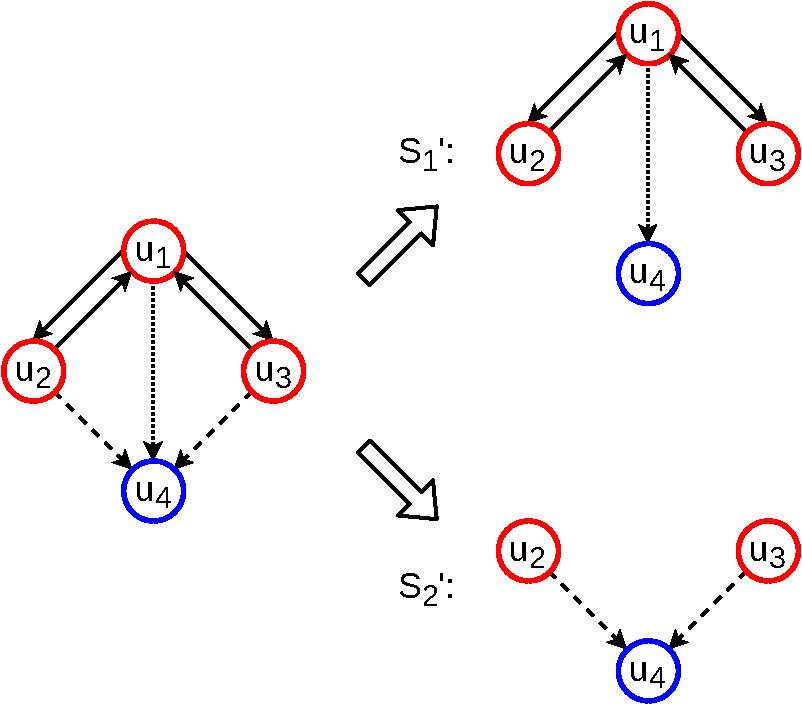
\includegraphics[width=0.35\textwidth]{img/stwig.pdf}
  \caption{Stars generated by existing algorithms.}\label{img:stwig}
\end{figure}
The edge $u_1 \rightarrow u_4$ is lost in $S_2'$.
Therefore, vertex $10$ will be matched (Figure~\ref{img:running_example}) which is unnecessary.
The problem is more severe for complex patterns where more edges need to be discarded.

SeqStar addresses the problem by keeping the original pattern graph unchanged, and removing vertices/edges on a copy $p'$ of the pattern (Algorithm~\ref{alg:decompose_stars}).
Algorithm~\ref{alg:decompose_stars} is similar to the vertex-cover selection algorithm~\cite{DBLP:books/daglib/0023376}.
The set $R$ in Algorithm~\ref{alg:decompose_stars} stores the candidate root vertices.
The algorithm uses a heuristic function $f(u) = \frac{\deg(u) + |\psi(u)|}{\operatorname{freq}(u.label)}$ to select roots,
where $\deg(u)$ is the degree of $u$, $|\psi(u)|$ is the number of constraints related to $u$ ($u_2 > u_1$, $u_3 > u_1$, $u_4 < 8$ in Figure~\ref{img:running_example}),
and $\operatorname{freq}(u.label)$ is the frequency of $u$'s label in the data graph.
By maximizing the function $f$,
SeqStar prefers vertex that
(1) has a high degree and has more associated constraints,
(2) has a less popular label in the data graph.
Therefore, the size of intermediate results from star matching can be reduced.
The neighbors of the selected root will then be added to the candidate set $R$.
By doing so, the roots selected by Algorithm~\ref{alg:decompose_stars} will be connected and forms a \emph{connected vertex-cover}.
And we'll use this property to build index for join operation~\ref{sec:match_join}.
Finally, SeqStar uses the selected root to extract stars from the original pattern graph $p$.
$\operatorname{Star}(p, root)$ is obtained by copying all the edges connected with $root$.
Therefore, all the structural information of $p$ is inherited to the stars.
%TODO:这里加讨论,这两条的点在之后的匹配中能够起到什么作用。

  %% Consider the pattern graph in Figure~\ref{img:star_decomposition},
  %% suppose that $u_1$, $u_2$ and $u_3$ are selected as the roots,
  %% existing decomposition method would result in three stars with 3, 2 and 1 neighbor\@(s)
  %% by consecutively selecting and removing vertices from the original pattern.
  %% However, many useful matching information are lost by doing so,
  %% e.g., the third ``star'' is just an edge, which would generate enormous unnecessary matching results whereas every edge in the data graph would match it but only a part of them could match the original pattern graph.
  %% In contrast, our approach (Algorithm~\ref{alg:decompose_stars}) would keep all the neighborhood matching information as is shown in the bottom of Figure~\ref{img:star_decomposition}, which could then reduce unnecessary intermediate results significantly (Section~\ref{sec:experiments}).
  %% Like previous work~\cite{DBLP:journals/pvldb/SunWWSL12}, we also use a heuristic function to select a join order, which is defined as $ f(u) = \frac{\deg(u) + |\psi(u)|}{\operatorname{freq}(u.label)} $, i.e.,
  %% we prefer to select vertex with bigger degree (more early filters) and less label frequency (smaller intermediate matching results) first.
  %% $|\psi(u)|$ is the number of local constraints of $u$, which will be discussed further in Section~\ref{sec:match_optimize}.
  %% The root candidate set $R$ is used to select a connected vertex cover,
  %% which could then be joined efficiently (Section~\ref{sec:match_join}).
  %% The key feature of the algorithm is to remove selected vertex in a copy $p'$ of the pattern and always keeps the original useful information in $p$, and thus, the intermediate results of our star could be much smaller.
  %% \begin{figure}[ht]
  %%   \centering
  %%   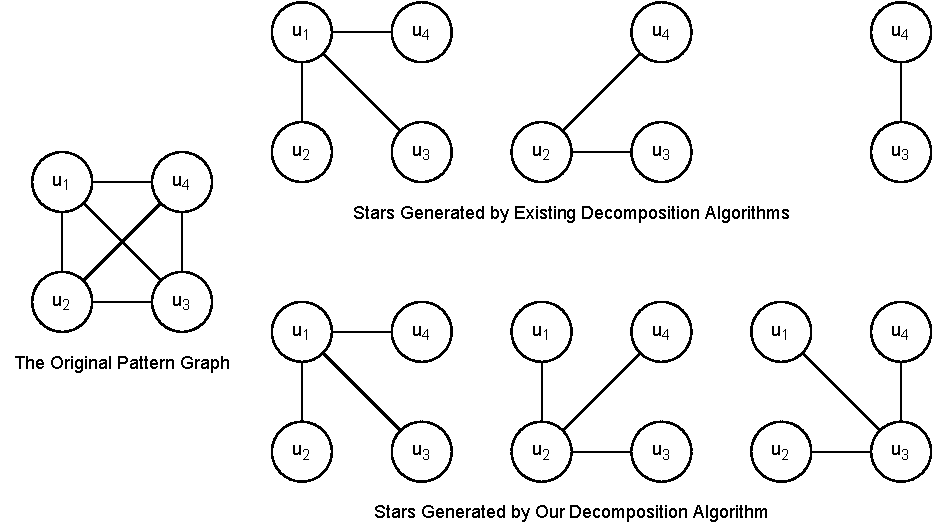
\includegraphics[width=0.48\textwidth]{img/star_decomposition.pdf}
  %%   \caption{Stars decomposed from the same pattern graph using different algorithms.}\label{img:star_decomposition}
  %% \end{figure}
%% \end{enumerate}
\begin{algorithm}[ht]
  \caption{Star Decomposition}\label{alg:decompose_stars}
  \SetKwFunction{DecomposeStars}{\textsc{DecomposeStars}}
  \SetKwFunction{Peek}{\textsc{Peek}}
  \SetKwFunction{Star}{\textsc{Star}}
  \SetKwFunction{RemoveVertex}{\textsc{RemoveVertex}}
  \Fn{\DecomposeStars{$p$}}{
    $stars \leftarrow \emptyset$\;
    $p' \leftarrow p$\;
    $R \leftarrow \{\max_{u \in V(p)}f(u)\}$\;
    \While{$R \neq \emptyset$}{
      $root \leftarrow \max_{u \in R}f(u)$\;
      $R \leftarrow R \setminus \{ root \}$\;
      $R \leftarrow R \cup \{ leaf \mid leaf \text{ is adjacent to } root \text{ in } p'\}$\;
      \RemoveVertex{$p'$, $root$}\;
      $R \leftarrow R \setminus \{ u \mid u \in p' \land \deg{u} = 0 \}$\;
      $stars \leftarrow stars \cup \{$ \Star{$p$, $root$} $\}$\;
    }
    \Return{$stars$}
  }
\end{algorithm}

To match a star $S$ on the vertex-centric storage engine,
SeqStar first seeks the \textsc{VertexIter} by searching the global index of the storage engine.
For each vertex $v$ in \textsc{VertexIter},
SeqStar first checks the degree of $v$ and applies constraints if available (\S\ref{sec:match_optimize}) to determine whether $v$ could be matched.
If $v$ passes these filters, SeqStar checks the neighbors of $v$ by visiting the \textsc{NeighborIter}.
For each neighbor vertex $n$ in \textsc{NeighborIter},
the in/out-edges associated with $n$ is compared to the corresponding leaf vertex of the star pattern.
The constraints extract from the WHERE clause will be applied to filter out unnecessary $n$ (\S\ref{sec:match_optimize}).
Since the iterators will only incur sequential data accesses,
the star matching process avoids the random disk seeks.

SeqStar adopts two techniques to further reduce the I/O cost:
(1) SeqStar analyzes the isomorphism among the stars to avoid redundant I/Os.
%% Some pattern may generate isomorphic stars, e.g., a triangle where each vertex has an edge point in and out.
Though the general graph isomorphism problem is NP complete, the isomorphism of stars are much easier to check.
We define an order for the vertices in a star based on the vertex labels. The isomorphism among stars can be checked by comparing the sorted stars.
Isomorphic stars have the same matching results. They only need to match once.
%and SeqStar will only match once for all.
(2) As the disk scanning operation is time consuming, it is preferable to scan it only once when solving a property graph matching problem.
SeqStar addresses the challenge by grouping stars with the same root label together,
and matches them in a single \textsc{VertexIter}.
For each scanned vertex $v$, SeqStar will check all the star patterns with the same root label as $v$.
Therefore, the graph data can be scanned only once without back and forth seeking.

%% Since the real-world graphs are so large that it is preferable to scan it only once when solving a property graph matching problem.
%% SeqStar solves the problem by grouping stars with the same root label together,
%% and scans these stars together by iterating through the \textsc{VertexIter}.
%% For each scanned vertex, SeqStar visits the \textsc{NeighborIter} to check the neighbors and stores the intermediate results for these stars.
%% Moreover, SeqStar is able to find isomorphism among stars and avoids unnecessary star matching (\S\ref{sec:match_optimize}).
%% However, it is not a simple task to match multiple stars in a single sequential scan,
%% the context switch cost and the intermediate result write cost must be minimized.
%% For the context switch cost, it is strongly coupled with the underlying storage method of the data graph.
%% Thanks to the elegant design of our vertex-centric storage model,
%% which is able to match stars in a sequential run given a root label,
%% we could group the stars with the same root label together and match them at the same time when iterating through \textsc{VertexIter}.
%% For the matching result write cost, we developed a compression algorithm for star's matching results that could be wrote sequentially (Section~\ref{sec:match_compress}).
%% As a result, we could scan the huge data graph only once and all the I/Os are sequential.

\subsection{Intermediate Results Compression}\label{sec:match_compress}
The matching results grow exponentially with respect to the size of the graph data.
%TODO:多次提到中间结果指数膨胀,最好在第一次出现的时候说点理由,从别人论文里面摘录出来也行
Consider the matching problem in Figure~\ref{img:running_example},
$S_1$ will generate 28 rows of intermediate results and $S_2$ will generate 8 rows.
And we need $4 \times (28 + 8) = 144$ integers to store them, which is larger than the data graph (10 vertices, 20 edges).
Inspired by the vertex-cover based compression algorithm~\cite{DBLP:journals/pvldb/QiaoZC17},
SeqStar postpones the costly Cartesian product and leveraging equivalence classes among vertices to reduce the size of intermediate results.
Moreover, we design an on-disk layout that is able to write the compressed data sequentially.

Two techniques are used to compress the intermediate results:
(1) Like VCBC, SeqStar avoids the Cartesian product in the intermediate results.
For each vertex $v$ that will match the root of a star $S$,
SeqStar stores the matched vertices of each neighbor of $v$ in $S$ together as an \emph{image set}.
They are then stored together as a \emph{SuperRow}.
For example, there are two SuperRows in $T_2$ (Figure~\ref{img:running_example}),
each contains a root vertex and two image sets.
(2) SeqStar analyzes the vertices in stars and use equivalence classes to avoid unnecessary storage.
SeqStar first groups the leaf vertices by label.
It then studies the connections between the leaves and the root.
Vertices have the same edge properties (direction, labels) and filtering function are grouped together as a \emph{neighbor equivalence class},
e.g., $u_2$ and $u_3$ in Figure~\ref{img:running_example}.
The matching results of the vertices are the same, and SeqStar stores their image set only once.
As a result, SeqStar uses only 16 integers to store the compressed intermediate results in Figure~\ref{img:running_example}.
\begin{figure}[ht]
  \centering
  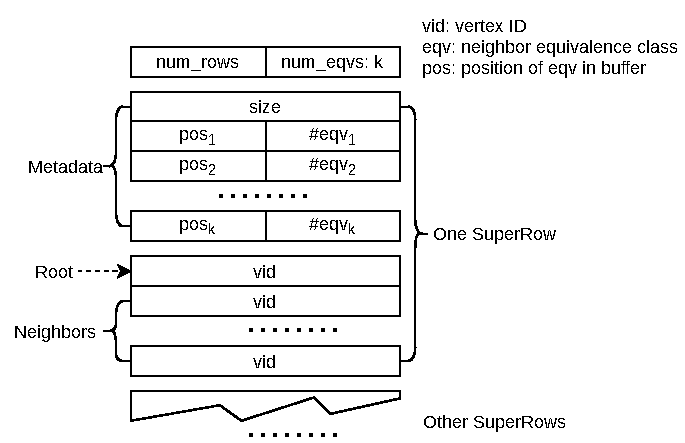
\includegraphics[width=0.45\textwidth]{img/compress.pdf}
  \caption{On-disk layout of the compressed intermediate results.}\label{img:compress}
\end{figure}

Figure~\ref{img:compress} shows the SuperRows' on-disk layout.
In each SuperRow, the matched vertices are stored consecutively.
Metadata $(pos_i, \#eqv_i)$, $ 1 \le i \le k$, are used to store the image sets for each neighbor equivalence class.

During the star matching process, matched vertices from the \textsc{NeighborIter} will be appended to the SuperRow file.

%% VCBC groups the matching results by the vertex-cover and stores the matched vertices in \emph{image sets}.
%% The original data can be restored by doing Cartesian product on the image sets.
%% As a result, only 16 integers are required
%% The compression ratio of the algorithm is as high as $10^{10}$ (\S\ref{sec:experiments_compress}).

% As our experiment shows that a small graph with $10^5$ edges could easily results in $10^{10}$ rows of matching results (Section~\ref{sec:experiments}).
%% Even though we could use stars and auxiliary optimizations to drop out useless matching results as soon as possible, the intermediate results could still be very large.
%% Figure~\ref{img:compress_example} illustrates this phenomenon that a small graph with only 6 vertices could result in 12 rows (48 vertices) of matching results.
%% In the table we could find that $u_1$ and $u_4$ always match the same vertices $v_2$ and $v_1$,
%% whereas the matching results of $u_2$ and $u_3$ are permutations of $v_3, v_4, v_5, v_6$.
%% \emph{The key of the matching result explosion problem is the explosive permutation}.
%% In order to address this problem, we avoid the permutation by postpone the Cartesian production when matching stars, which is similar to VCBC~\cite{DBLP:journals/pvldb/QiaoZC17} but we focus on the compression of property star's matching results for out-of-core systems.

%% Consider Figure~\ref{img:compress_example}, there is a symmetry with $u_2$ and $u_3$.
%% We say that they have the same \textsc{NeighborInfo} or they form a \textsc{NeighborInfo} equivalence class, as they have the same label and same connections to the root $u_4$,
%% and we can be sure that the matching results of $u_2$ and $u_3$ are always same.
%% The \textsc{NeighborInfo} of $u_1$ is different from $u_2$ because $u_1$ has more edges connected to the root.
%% By iterating through the neighbors of $v_1$, we can find the image set for each vertex in the pattern.
%% Instead of permuting the matching vertices, we compress the matching result by just writing down the image sets of each \textsc{NeighborInfo} equivalence class as is shown in the right bottom corner in Figure~\ref{img:compress_example}.
%% And Figure~\ref{img:compress} gives a straightforward disk format to store the compressed star matching results.
%% The final results can be retrieved by doing Cartesian product on the image sets and keeping the unique vertices.
%% We called the compressed data as \emph{SuperRow} since one SuperRow could generate enormous tuples by Cartesian production.
%% \begin{figure}[ht]
%%   \centering
%%   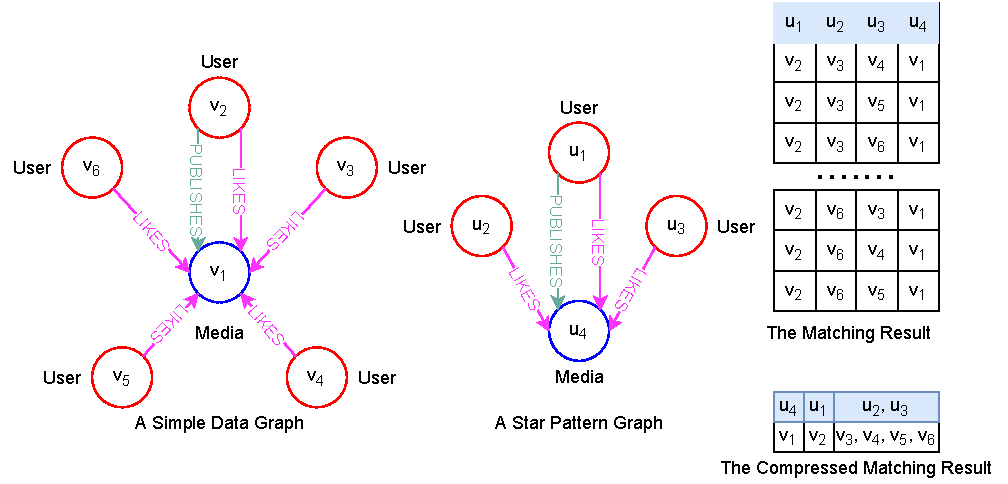
\includegraphics[width=0.53\textwidth]{img/compress_example.pdf}
%%   \caption{A small graph could results in enormous matching results.}\label{img:compress_example}
%% \end{figure}

%% However, there are still two challenges to be faced in practice:
%% 1. In real-world property graphs, as a celebrity vertex could have millions of neighbors, it could become a bottleneck if we have to scan the neighbors multiple times when matching a star;
%% 2. The SuperRows should be written sequentially to reduce the I/O cost.
%% If we want to scan the neighbors only once, we should be able to append the neighbor vertex to the corresponding image set, however, the variable-length image sets make it hard to address these problems.
%% To solve this dilemma, for each SuperRow, we pre-allocate enough space based on the statistical information in the data graph, i.e., the size of neighbors with the \textsc{NeighborInfo}'s label.
%% Thus the vertices could be scanned only once and wrote to the corresponding image set sequentially.

\subsection{Pipeline Join on Compressed Data}\label{sec:match_join}
%% By far, we've got all the compressed matching results for stars and it's time to join them to obtain the final answer.
%% A simple and straightforward method is the binary join, however, intermediate join results have to be materialized by doing so.
%% Even though the compression ratio of star matching result is very impressive,
%% the joined result could expand significantly because the permutation among roots is unavoidable~\cite{DBLP:journals/pvldb/SunWWSL12}.
%% To address this problem, we propose a indexed pipeline join algorithm on compressed data:
SeqStar reduces the memory usage further by performing pipeline join on compressed data.

To boost the join operation, we design an index on the SuperRow data.
Consider the SuperRow layout in Figure~\ref{img:compress}, each SuperRow contains only one root.
The uniqueness of the root makes it possible to be the key of a index (SuperRow-index):
Given a root ID, it returns the position of the corresponding SuperRow.
Since the vertices are sorted in the storage engine,
the SuperRow-index can be build by appending after a SuperRow is stored.
And the SuperRow-index operates by a simple binary search.

The planner of SeqStar first generate a join order based on the statistical parameters of SuperRows,
i.e., row number, average size of image sets.
The parameters are accumulated when a SuperRow is appended, and the cost is trivial.
Also note that in Algorithm~\ref{alg:decompose_stars}, the chosen root vertices form a connected vertex-cover.
The join order ensures the root of the stars are bound by previous stars.
For example, $T_1 \Join T_2 \Join \cdots \Join T_c$ (the discussion can be generalized to other join orders),
where $T_i$ is the SuperRows of $S_i$, and the root of $S_i$ is $u_i$.
SeqStar ensures $u_i \in V(S_{i-1})$ such that the Super-indexes will always work.

After that, SeqStar performs a pipeline join on the SuperRows to avoid materializing intermediate results.
The basic structure of the algorithm is a series of nested loops  (Algorithm~\ref{alg:join}).

\begin{algorithm}[ht]
  \caption{Pipeline Join}\label{alg:join}
  \SetKw{Yield}{yield}
  \ForEach{$sr_1 \in T_1$}{
    $v_1 \leftarrow sr_1[u_1]$\;
    \ForEach{$v_2 \in sr_1[u_2]$}{
      \If{$sr_2 \leftarrow T_2.idx(v_2)$}{
        \ForEach{$v_3 \in \bigcap_{u_3 \in sr}sr[u_3]$}{
          $\cdots$\;
          \If{$sr_c \leftarrow T_c.idx(v_c)$}{
            \Yield{$(v_1, \dots, v_c, \bigcap_{u_{c+1}\in sr}sr[u_{c+1}], \dots)$}\;
          }
        }
      }
    }
  }
\end{algorithm}

Unlike the traditional join problem, SeqStar joins on image sets rather than single elements.
That is to say set intersection is the most computation-intensive operation.
Since vertices are sorted in the storage engine,
the order will still preserves in every image sets.
This property makes it perfect for the merge algorithm to perform set intersection.
%% Consider the SuperRows in Figure~\ref{img:running_example}, whose columns are image set for \textsc{NeighborInfo} equivalence class except the first column, which is the matching result of the root.
%% Thus the first column of a SuperRow contains only a single vertex, which is suitable for the key of a index.
%% In fact, the index is generated during the star matching process,
%% for each SuperRow we append the root id and the position of it to the index file.
%% With this index, we are able to locate to the corresponding SuperRows efficiently during the join process.

%% The basic structure of our pipeline join is a series of nested loops.
%% However, unlike the traditional join problem, we join on image sets rather than single elements,
%% which means set intersection is the most computation intensive operation.
%% Consider the social media network, a trending media could easily attract millions or even billions of viewers,
%% to join on such trending media rooted stars, we must calculate the set intersection of such enormous viewers.
%% A conventional hash join method could easily eat up the memory of a PC and have poor locality.
%% To address this problem, we provide an out-of-core sequential approach by merging on the image sets.
%% Therefore the image sets should be sorted otherwise the sorting operation could be another bottleneck.
%% In fact, with the elegant design of our vertex-centric property graph storage method,
%% the vertices are already sorted in the data graph, and we can implement our sequential out-of-core set intersection for free.

\subsection{Optimizations}\label{sec:match_optimize}
In this section we discuss a series of optimizations for the property graph matching engine.
\subsubsection{Predicate Push Down}
The WHERE clause of a graph matching query specified a constraint or searching condition on the matching results.
The constraint are expressed in the form of predicates, e.g., $=$, $\neq$, $>$, $\ge$, $<$, $\le$.
And the Boolean operator AND ($\land$), OR ($\lor$), NOT ($\lnot$) can be used to combine multiple predicates into a new one.
For example, in Figure~\ref{img:cypher_query}, there are three predicates concatenated by AND\@.
Formally, the constraint is a function $\psi: PG \rightarrow B$ with $PG$ the set of pattern graph and $B$ the set of Boolean values.
We will also use $\psi$ to denote abstract predicate for simplicity in this section:
$\psi(u)$ defines a constraint $\psi$ on vertex $u$, e.g., ``{id(u4) >= 2020}'' defines a vertex constraint on $u_4$ where the ID of the matching vertex of $u_4$ must great than or equal to $2020$;
and $\psi(u_1, u_2)$ defines a constraint on vertex $u_1$ and vertex $u_2$,
e.g., ``{id(u1) < id(u2)}'' defines a constraint on $u_1$ and $u_2$ that the ID of the matching of $u_1$ must be less than that of $u_2$.

Previous work usually ignore the constraint specification part of a graph matching query.
If someone wants to query a pattern with a specific searching condition,
she or he has to match the pattern graph first and then filter on the matching results,
which leaves a lot of room for improvement because the user provided searching conditions could filter out many unnecessary
partial results in an early phase.

However, it is still challenging to make use of the constraint provided by user's WHERE clause.
The pattern graph and the constraint are logically two different things,
we have to obtain enough information in order to use the constraint as early filter during the graph matching phase.
For example, the constraint in Figure~\ref{img:cypher_query} include all the vertices in the pattern graph,
only when the pattern graph is already matched could we got enough information to apply the constraint,
which makes the constraint filter nearly useless.

\begin{figure}[ht]
  \centering
  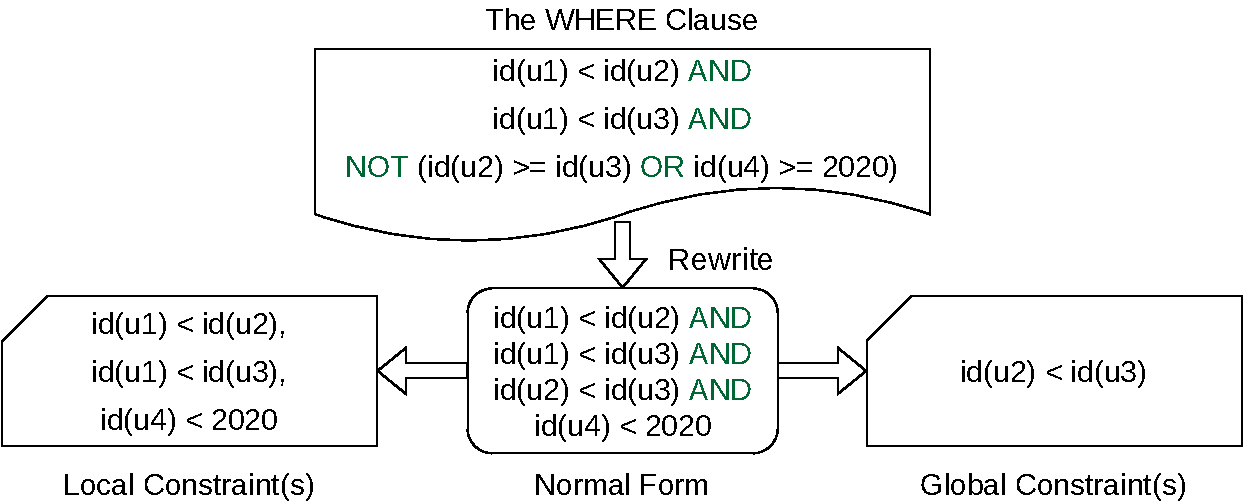
\includegraphics[width=.45\textwidth]{img/constraints.pdf}
  \caption{Constraint Analysis.}\label{img:constraints}
\end{figure}

To address this problem, as shown in Figure~\ref{img:constraints},
we dive into the syntax tree of the graph matching query and decompose the searching condition into smaller parts which require only what we could got during the graph matching phase.
Specifically, we decompose the searching condition into three parts: \emph{vertex constraints}, \emph{edge constraints} and \emph{global constraint}.
A vertex constraint is a function $\psi(u)$ mapping vertex $u$ to Boolean values,
and an edge constraint sets a constraint on edge $(u_1, u_2)$ by a function $\psi(u_1, u_2)$.
For example, in Figure~\ref{img:pattern_graph} ``{id(u4) < 2020}'' sets a vertex constraint on $u_4$,
``{id(u1) < id(u2)}'' and ``{id(u1) < id(u3)}'' are edge constraints,
while ``{id(u2) < id(u3)}'' is not because there is no edge between $u_2$ and $u_3$.
The \emph{vertex constraints} and \emph{edge constraints} are \emph{local constraints} that only require local information that can be obtained during the graph matching phase.
So they could then be pushed down to the data graph scanning phase to short-circuit useless matching results.
A global constraint $\psi(u_1, u_2, \dots)$ sets a constraint on a series of vertices $u_1, u_2, \dots$,
the information is insufficient during the data graph scanning phase.

\begin{algorithm}[ht]
  \caption{Constraint Rewriting}\label{alg:rewrite}
  \SetKwFunction{ConstraintRewrite}{\textsc{ConstraintRewrite}}
  \SetKwFunction{Simplify}{\textsc{Simplify}}
  \Input{$expr$: the abstract syntax tree of the WHERE clause}
  \Output{A set of simplified constraints connected by the AND ($\land$) operator}
  \Fn{\ConstraintRewrite{$expr$}}{
    \Match{$expr$}{
      \Case{$\lnot \lnot e$}{\Return{\ConstraintRewrite{$e$}}}
      \Case{$\lnot (e_1 \lor e_2)$}{
        \Return{\ConstraintRewrite{$\lnot e_1$} $\cup$ \ConstraintRewrite{$\lnot e_2$}}
      }
      \Case{$e_1 \land e_2$}{\Return{\ConstraintRewrite{$e_1$} $\cup$ \ConstraintRewrite{$e_2$}}}
      \Case{$e$}{\Return{$\{$ \Simplify{$e$} $\}$}}
    }
  }
\end{algorithm}

Logically, the AND ($\land$) operator create a new constraint $\psi = \psi_1 \land \psi_2$ by combining two constraints $\psi_1$ and $\psi_2$,
where $\psi_1$ and $\psi_2$ can be used to check the matching results independently because there is no side effects in constraints,
so we could safely split $\psi$ into $\psi_1$ and $\psi_2$.
Because local constraints are the earliest constraint filters, we should extract as much as possible.
In order to make the constraint filters more efficient and extract more local constraints:
Firstly, we optimize the AST by classic methods such as compile-time calculation,
handle special cases such as ``{WHERE false}''.
Then, we apply Algorithm~\ref{alg:rewrite} to analyze the syntax tree and rewrite it into \emph{normal form},
where a normal form is a list of simplified constraints connected by the AND operator.
In fact, the constraints are mostly specified by binary operators such as ``$\le$'', ``$\ne$'',
hence many constraints are naturally local constraints.
And the De Morgan's law enables us to convert the OR ($\lor$) operator into AND ($\land$):
\begin{equation}
  \lnot (\psi_1 \lor \psi_2) = \lnot \psi_1 \land \lnot \psi_2
\end{equation}
So Algorithm~\ref{alg:rewrite} will always keep the semantics of the original user provided constraint.
For example, the third predicate of the AND operator in Figure~\ref{img:cypher_query} would be rewritten to
\begin{verbatim}
  id(u2) < id(u3) AND id(u4) < 2020
\end{verbatim}
by applying De Morgan's law.
And the WHERE clause of Figure~\ref{img:cypher_query} would be rewritten to the normal form:
\begin{verbatim}
  WHERE id(u1) < id(u2) AND id(u1) < id(u3)
  AND id(u2) < id(u3) AND id(u4) < 2020
\end{verbatim}

\begin{algorithm}[ht]
  \caption{Constraint Pushdown}\label{alg:push_down}
  \SetKwFunction{ConstraintPushdown}{\textsc{ConstraintPushdown}}
  \SetKwFunction{AddVertexConstraint}{\textsc{AddVertexConstraint}}
  \SetKwFunction{AddEdgeConstraint}{\textsc{AddEdgeConstraint}}
  \SetKwFunction{Edges}{\textsc{Edges}}
  \Input{The normal form of constraints $exprs$ and the user described pattern graph $p$}
  \Output{The vertex constraints and edge constraints are pushed down to $p$ and the global constraints will be returned}
  \Fn{\ConstraintPushdown{$exprs$, $p$}}{
    $globals \leftarrow [\,]$\;
    \ForEach{$expr \in exprs$}{
      \Match{$expr$}{
        \Case{$\psi(u)$}{\AddVertexConstraint{$p$, $\psi(u)$}}
        \Case{$\psi(u_1, u_2)$}{
          \If{$(u_1, u_2) \in$ \Edges{$p$}}{\AddEdgeConstraint{$p$, $u_1$, $u_2$, $\psi(u_1, u_2)$}}
        }
        \Case{$e$}{$globals \leftarrow globals \cup \{e\}$\;}
      }
    }
    \Return{$globals$}
  }
\end{algorithm}

The normal form is then used to extract useful information to be pushed down to the pattern graph as in Algorithm~\ref{alg:push_down}.
For each constraint in the normal form, we check if it is local constraint and then push it down to the corresponding vertex or edge.
After that, We could then decompose it into stars.
Our framework contains a JIT compiler that is able to emit callable closures based on the AST,
and the local constraints can then be used to serve as early filters in the data graph scanning process to short-circuit unnecessary matchings as soon as possible.
\subsubsection{Star Isomorphism}
Consider Figure~\ref{img:star_decomposition}, we generate three stars from the original pattern,
and these stars are isomorphic with each other.
Therefore the matching results of these stars are always the same,
there is no need to match these stars again and again.
Though the general graph isomorphism problem is NP complete,
the isomorphism of stars are easier to check.
We say that our stars in Figure~\ref{img:star_decomposition} belong to the same \textsc{Characteristic} equivalence class,
where \text{Characteristic} is a structure that stores the root and neighbors in a predefined order.
By grouping isomorphic stars into the same \textsc{Characteristic} equivalence class,
we could avoid unnecessary computation.

